\section{Spiking Neural Networks}
\label{sec:background_snn}

\glspl{snn} represent a fundamentally different computational paradigm to the standard \gls{ann} architectures described in the preceding sections.
Rather than propagating continuous-valued activations between layers, \glspl{snn} communicate exclusively through discrete binary events, spikes, mimicking the all-or-nothing firing behaviour of biological neurons \cite{Roy2019SpikeBasedMI}.
By prioritising event-driven binary communication, this paradigm aims to drastically reduce both dynamic power consumption and computational complexity compared to traditional deep learning models, making it inherently suited to power and latency-constrained environments.

\subsection{The Leaky Integrate-and-Fire Neuron}
\label{subsec:bg_lif}

At the foundation of most practical \glspl{snn} lies the \acrfull{lif} neuron model, which governs the temporal dynamics and binary spike generation of the network.
Unlike standard \glspl{ann} that utilise continuous activation functions such as \gls{relu}, the \gls{lif} node maintains an internal state: the membrane potential $V[t]$, which updates iteratively across discrete timesteps $t \in [1, T]$.

The dynamics of the \gls{lif} neuron at a given spatial position and timestep $t$ are governed by the integration of incoming pre-synaptic spatial features $X[t]$ and an inherent leak factor $\tau$, which dictates how quickly $V[t]$ returns to its resting state in absence of incoming input.
The hidden membrane potential $H[t]$ prior to spiking is mathematically defined as:
\begin{equation}
    H[t] = V[t-1] + \frac{1}{\tau} \left(X[t] - (V[t-1] - V_{reset})\right)
\end{equation}
When $H[t]$ exceeds a predefined threshold $V_{th}$, the neuron emits a binary spike $S[t] \in \{0, 1\}$ to the subsequent layer, governed by the Heaviside step function $\Theta(x)$:
\begin{equation}
    S[t] = \Theta(H[t] - V_{th})
\end{equation}
Following a spike ($S[t]=1$), the neuron undergoes a hard reset, instantly dropping its potential $V[t]$ to $V_{reset}$, mimicking the refractory period of biological neurons, preventing infinite spiking and overstimulation \cite{sarpeshkar1992refractory}.
If no spike is emitted ($S[t]=0$), the potential naturally decays, ensuring that subsequent layers only perform computations upon receiving active events \cite{sengupta2019goingdeeperspikingneural}.
This \textit{activation sparsity}: the property that computation is only triggered by genuine signal, not by silence, which is the primary driver of the \gls{snn}'s exceptional energy efficiency \cite{Roy2019SpikeBasedMI} --- where a \gls{cnn} triggers computation regardless of the input stimuli, an \gls{snn} only triggers synaptic operations in response to discrete spikes, effectively idling during periods of silence.

\subsection{Surrogate Gradients}
\label{subsec:bg_surrogate}

Training deep \glspl{snn} via backpropagation presents a fundamental mathematical challenge, since the Heaviside step function governing spike generation is non-differentiable.
As established in Section~\ref{sec:background_ann}, the chain rule requires every function in the computational graph to be differentiable; the Heaviside function violates this directly, since its derivative is zero everywhere except at the threshold $V_{th}$, where it is infinite.
Using conventional backpropagation therefore results in zeroed gradients that immediately halt the learning process, a phenomenon known as the ``dead neuron'' problem.

To resolve this, \glspl{snn} employ a \textit{surrogate gradient} during the backward pass \cite{nfetci2019_surrogate}.
While the forward pass remains strictly binary, the backward pass approximates the step function using a smooth, differentiable curve.
A common choice is the \gls{atan} function:
\begin{equation}
    \frac{\partial S}{\partial H} \approx \frac{\alpha}{2\left(1 + \left(\frac{\pi}{2} \alpha (H - V_{th})\right)^2\right)}
\end{equation}
where $\alpha$ is a hyperparameter controlling the steepness of the surrogate curve.
This mathematical substitution allows the network to learn complex spatiotemporal representations from scratch while maintaining a purely binary forward execution, with gradients propagated through the temporal dimension via \acrfull{bptt}.

\subsection{Spike-Element-Wise Residual Blocks}
\label{subsec:bg_sew}

Building deep \glspl{snn} introduces a further challenge beyond the surrogate gradient problem: the \textit{vanishing spike} problem inherent in standard residual connections.
In a standard \gls{resnet} (Section~\ref{sec:background_cnn}), the residual addition occurs before the activation function.
However, applying this directly to a spiking network causes a critical failure, because adding two binary spike trains produces a non-binary, continuous value (e.g., $1 + 1 = 2$), which destroys the energy-efficient, event-driven nature of the network \cite{fang2022resnet_sew}.

To overcome this, \textcite{fang2022resnet_sew} proposed the \acrfull{sew} residual paradigm, instantiated as \texttt{SEWResBlock} units.
Unlike standard Spiking ResNets, \gls{sew} ResBlocks apply the element-wise residual operation after the spiking activation function, guaranteeing that the output remains strictly binary.
\textcite{fang2022resnet_sew} proved that this reordering is both necessary and sufficient to achieve identity mapping in a purely spike-based network, resolving the vanishing spike problem and enabling representational depth that would otherwise induce spike degradation.

\begin{figure}[h]
    \centering
    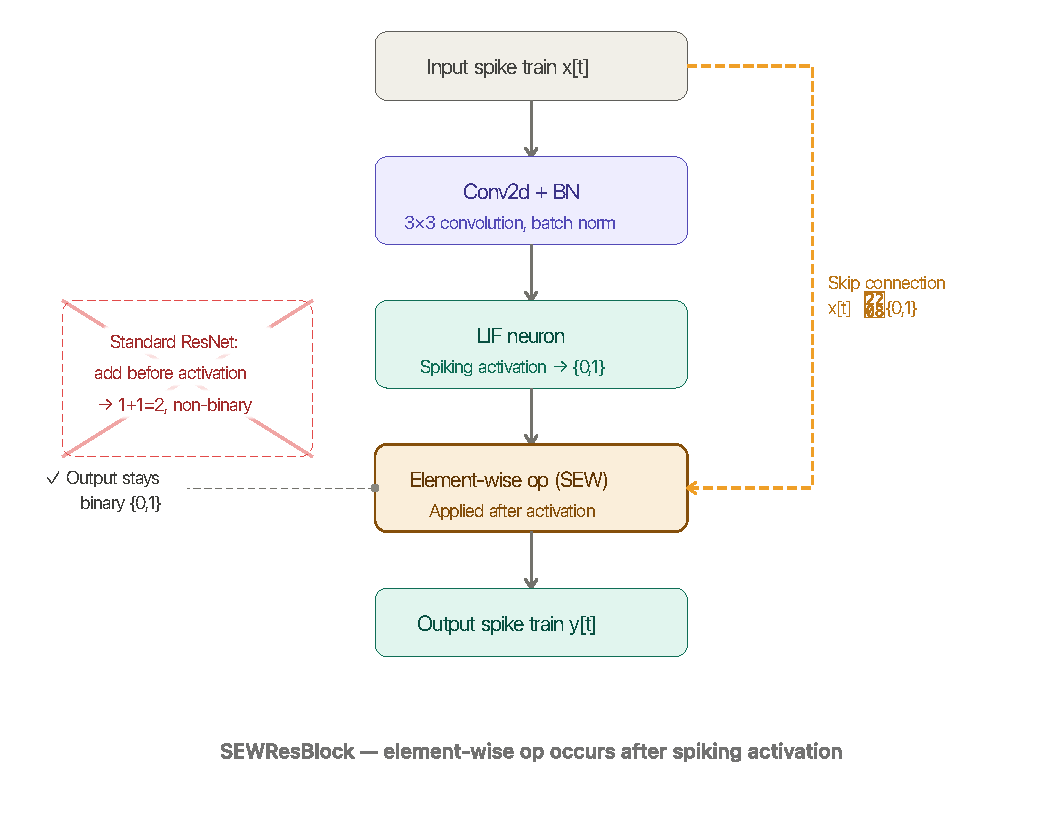
\includegraphics[width=0.9\textwidth]{chapter_3/figures/sewresblock_diagram.pdf}
    \caption[SEW Residual Block]{The \gls{sew} residual block (\texttt{SEWResBlock}) as proposed by \textcite{fang2022resnet_sew}.}
    \label{fig:sewresblock_bg}
\end{figure}

\clearpage

\subsection{Temporal Dynamics \& Rapid Categorisation}
\label{subsec:bg_temporal}

A defining property of \glspl{snn} is their natural ability for spatiotemporal integration, combining timing and location when processing information.
By processing an event stream iteratively across $T$ discrete timesteps, an \gls{snn} is capable of producing meaningful predictions before the full observation window has elapsed \cite{pfeiffer_snn_opportunities}.
This property is absent in a standard \gls{cnn}, which performs a single spatial pass over the fully integrated input and can only produce an output once all temporal evidence has been collected.

This progressive refinement is analogous in spirit to the \textit{rapid categorisation} phenomenon documented in the human visual system, where early feedforward spikes drive coarse semantic decisions that sharpen as further neural evidence accumulates \cite{thorpe1996speed}.
While \textcite{thorpe1996speed} address categorical recognition rather than coordinate regression, the underlying principle that sparse early spike activity produces meaningful but imprecise representations which sharpen over time is directly consistent with the anticipated behaviour of a spiking detection backbone.

\todo[inline]{Can refer to this in 3.7.4}

Rate coding over a fixed window of $T$ timesteps carries an inherent representational limit known as the "quantisation error"; the precision of the encoded signal is bounded by a $1/T$ quantisation floor, since information is encoded as spike counts that can take only $T+1$ discrete values \cite{THORPE2001715}.
Alternative temporal coding schemes have been proposed to overcome this ceiling, including \acrfull{ttfs} encoding, where information is represented by the arrival time of the first spike rather than the firing frequency, and \acrfull{roc}, which represents signal intensities via relative firing orders and sub-millisecond arrival times \cite{THORPE2001715}.

\todo[inline]{\texttt{3\_4\_snn\_architecture.tex} §Neuron Dynamics: LIF --- strip all equations and mechanistic explanation. Retain only project-specific parameters ($V_{th}=0.2$, hard reset, $\tau$) and add a back-reference: ``the \gls{lif} model, as defined in Section~\ref{subsec:bg_lif}, governs the temporal dynamics of the network''.}

\todo[inline]{\texttt{3\_4\_snn\_architecture.tex} §Backward Pass --- strip the opening ``dead neuron'' motivation paragraph (covered in Sections~\ref{sec:background_ann} and~\ref{subsec:bg_surrogate}). Retain only the \gls{atan} equation and the project-specific $\alpha$ hyperparameter value, with a back-reference to Section~\ref{subsec:bg_surrogate}.}

\todo[inline]{\texttt{3\_4\_snn\_architecture.tex} §SEW-ResBlocks --- strip the vanishing spike explanation and remove the duplicate \texttt{sewresblock\_diagram.pdf} figure (now in Figure~\ref{fig:sewresblock_bg}). Reduce the intro to: ``as detailed in Section~\ref{subsec:bg_sew}, \gls{sew} ResBlocks resolve the vanishing spike problem by placing the residual operation after the spiking activation function \cite{fang2022resnet_sew}''.}

\todo[inline]{\texttt{3\_7\_sections/temporal\_evidence.tex} §Hypothesis: Bounding Box Sharpening --- strip the Thorpe rapid categorisation paragraphs (transferred to Section~\ref{subsec:bg_temporal}). Reduce to one sentence establishing the sharpening hypothesis, then proceed directly to the experimental methodology.}
